%%%%%%%%%%%%%%%%%%%%%%%%%%%%%%%%%%%%%%%%%%%%%%%%%%%%%%%%%%%%%%%%%%%%%%%%%%%%%%%%%%%%%%%%%%%%%%%%%%%%%%%
%%%%%%%%%%%%%% Template de Artigo Adaptado para Trabalho de Diplomação do ICEI %%%%%%%%%%%%%%%%%%%%%%%%
%% codificação UTF-8 - Abntex - Latex -  							     %%
%% Autor:    Fábio Leandro Rodrigues Cordeiro  (fabioleandro@pucminas.br)                            %% 
%% Co-autor: Prof. João Paulo Domingos Silva, Harison da Silva e Anderson Carvalho                   %%
%% Revisores normas NBR (Padrão PUC Minas): Helenice Rego Cunha e Prof. Theldo Cruz                  %%
%% Versão: 1.1     18 de dezembro 2015                     	                                     %%
%%%%%%%%%%%%%%%%%%%%%%%%%%%%%%%%%%%%%%%%%%%%%%%%%%%%%%%%%%%%%%%%%%%%%%%%%%%%%%%%%%%%%%%%%%%%%%%%%%%%%%%


\documentclass[a4paper,12pt,Times]{article}
\usepackage{abakos}  %pacote com padrão da Abakos baseado no padrão da PUC

%%%%%%%%%%%%%%%%%%%%%%%%%%%
%Capa da revista
%%%%%%%%%%%%%%%%%%%%%%%%%%

%\setcounter{page}{80} %iniciar contador de pagina de valor especificado
\newcommand{\monog}{A Lógica da Investigação Científica: Um Percurso pelos Três Tipos de Pesquisa}
\newcommand{\monogES}{Article template Institute of Mathematical Sciences and Informatics}
\newcommand{\tipo}{Artigo }  % Especificar a seção tipo do trabalho: Artigo, Resumo, Tese, Dociê etc
\newcommand{\origem}{Brasil }
\newcommand{\editorial}{Belo Horizonte, p. 01-11, nov. 2015}  % p. xx-xx – páginas inicial-final do artigo
\newcommand{\lcc}{\scriptsize{Licença Creative Commons Attribution-NonCommercial-NoDerivs 3.0 Unported}}

%%%%%%%%%%%%%%%%%INFORMAÇÕES SOBRE AUTOR PRINCIPAL %%%%%%%%%%%%%%%%%%%%%%%%%%%%%%%
\newcommand{\AutorA}{1543726 - Pedro Henrique Cardoso Maia}
\newcommand{\funcaoA}{}
\newcommand{\emailA}{pedro.maia.1543726@sga.pucminas.br}
\newcommand{\cursA}{Aluno do Programa de Graduação em Ciência da Computação}

% 
% Definir macros para o nome da Instituição, da Faculdade, etc.
\newcommand{\univ}{Pontifícia Universidade Católica de Minas Gerais}

\newcommand{\keyword}[1]{\textsf{#1}}

\begin{document}
% %%%%%%%%%%%%%%%%%%%%%%%%%%%%%%%%%%
% %% Pagina de titulo
% %%%%%%%%%%%%%%%%%%%%%%%%%%%%%%%%%%

\begin{center}

\includegraphics[scale=0.2]{figuras/brasao.jpg} \\
PONTIFÍCIA UNIVERSIDADE CATÓLICA DE MINAS GERAIS \\
Instituto de Ciências Exatas e de Informática

% \vspace{1.0cm}

\end{center}

 \vspace{0cm} {
 \singlespacing \Large{\monog \symbolfootnote[1]{Artigo apresentado ao Instituto de Ciências Exatas e Informática da Pontifícia Universidade Católica de Minas Gerais como pré-requisito para obtenção do título de Bacharel em Ciência da Computação.} \\ }
  \normalsize{\monogES}
 }

\vspace{1.0cm}

\begin{flushright}
\singlespacing 
\normalsize{\AutorA \footnote{\funcaoA \cursA, \origem -- \emailA . }} \\

\newcommand{\AutorB}{Author Name}

%\normalsize{\AutorC \footnote{\funcaoC \cursC, \origem -- \emailC . }} \\
%\normalsize{\AutorD \footnote{\funcaD \cursD, \origem -- \emailD . }} \\
%deixar com o valor `0` e usar o '*' no inicio da frase
% \symbolfootnote[0]{Artigo recebido em 10 de julho de 1983 e aprovado em 29 de maio 2012}
\end{flushright}
\thispagestyle{empty}

\vspace{1.0cm}

\begin{abstract}
\noindent
Este artigo discute os três tipos lógicos principais de pesquisa científica: exploratória, descritiva e explicativa. A pesquisa exploratória tem como objetivo oferecer uma compreensão mais profunda sobre um problema pouco estudado, servindo como fundamento para a construção de teorias e hipóteses. Por outro lado, a pesquisa descritiva se concentra na observação, registro, análise e interpretação de fenômenos sem intervenção direta, buscando retratar as características de um grupo ou contexto específico. A pesquisa explicativa, por sua vez, busca identificar as causas dos fenômenos, estabelecendo relações de causa e efeito entre diferentes variáveis. Entender as particularidades desses tipos de pesquisa é crucial para o desenvolvimento de um delineamento metodológico apropriado, assegurando a validade científica e a aplicabilidade prática dos estudos. Este trabalho, portanto, tem como objetivo contribuir para uma melhor compreensão dos processos de investigação científica, fundamentais para a produção acadêmica de qualidade.
\\\textbf{\keyword{Palavras-chave: }} Template. \LaTeX. Pesquisa, Exploratória, Descritiva.
\end{abstract}

%%%%%%%%%%%%%%%%%%%%%%%%%%%%%%%%%%%%%%%%%%%%%%%%%%%%%%%%%
 \newpage    %%%% CASO QUEIRA QUE O RESUMO FIQUE EM UMA PAGINA E O ABSTRACT EM OUTRA
\selectlanguage{english}
\begin{abstract}
\noindent
This article discusses the three main logical types of scientific research: exploratory, descriptive and explanatory. Exploratory research aims to provide a deeper understanding of a little-studied problem, serving as a basis for the construction of theories and hypotheses. On the other hand, descriptive research focuses on the observation, recording, analysis and interpretation of phenomena without direct intervention, seeking to portray the characteristics of a specific group or context. Explanatory research, in turn, seeks to identify the causes of phenomena, establishing cause and effect relationships between different variables. Understanding the particularities of these types of research is crucial for the development of an appropriate methodological design, ensuring the scientific validity and practical applicability of studies. This work, therefore, aims to contribute to a better understanding of the processes of scientific investigation, fundamental for quality academic production.
\\\textbf{\keyword{Keywords: }} Template. \LaTeX. Research, exploratory, descriptive.
\end{abstract}

\selectlanguage{brazilian}
 \onehalfspace  % espaçamento 1.5 entre linhas
 \setlength{\parindent}{1.25cm}

%%%%%%%%%%%%%%%%%%%%%%%%%%%%%%%%%%%%%%%%%%%%%%%%%
%% INICIO DO TEXTO
%%%%%%%%%%%%%%%%%%%%%%%%%%%%%%%%%%%%%%%%%%%%%%%%%

%%%%%%%%%%%%%%%%%%%%%%%%%%%%%%%%%%%%%%%%%%%%%%%%%%%%%%%%%%%%%%%%%%%%%%%%%%%%%%%%%%%%%%%%%%%%%%%%%%%%%%%
%%%%%%%%%%%%%% Template de Artigo Adaptado para Trabalho de Diplomação do ICEI %%%%%%%%%%%%%%%%%%%%%%%%
%% codificação UTF-8 - Abntex - Latex -  							     %%
%% Autor:    Fábio Leandro Rodrigues Cordeiro  (fabioleandro@pucminas.br)                            %% 
%% Co-autores: Prof. João Paulo Domingos Silva, Harison da Silva e Anderson Carvalho		     %%
%% Revisores normas NBR (Padrão PUC Minas): Helenice Rego Cunha e Prof. Theldo Cruz                  %%
%% Versão: 1.1     18 de dezembro 2015                                                               %%
%%%%%%%%%%%%%%%%%%%%%%%%%%%%%%%%%%%%%%%%%%%%%%%%%%%%%%%%%%%%%%%%%%%%%%%%%%%%%%%%%%%%%%%%%%%%%%%%%%%%%%%

\section{\esp OBJETIVO}

O objetivo central deste trabalho é realizar uma sistematização teórica e crítica dos três tipos lógicos de investigação — exploratória, descritiva e explicativa — enfatizando suas definições, metas específicas, métodos frequentemente empregados, áreas de aplicação e restrições. Com isso, busca-se proporcionar ao pesquisador iniciante e ao acadêmico mais experiente um referencial conceitual claro e prático para a escolha fundamentada do tipo de pesquisa que melhor se adapte às exigências de seus projetos. Além disso, pretende-se examinar como cada tipo lógico de investigação contribui para o processo de formulação de hipóteses, organização de dados empíricos e explicação científica, ressaltando sua relevância no rigor metodológico e na validação dos resultados obtidos na pesquisa.

\section{\esp DISCUSSÃO}

Os três tipos lógicos de pesquisa possuem propósitos e estratégias metodológicas distintas, embora possam ser utilizados de maneira complementar em investigações mais complexas.

A pesquisa exploratória destina-se ao reconhecimento de fenômenos ainda pouco conhecidos, sendo empregada principalmente quando não há hipóteses definidas ou modelos consolidados. Ela se caracteriza pela flexibilidade de métodos, como revisão bibliográfica ampla, entrevistas com especialistas e observação informal, permitindo ao pesquisador formular perguntas de pesquisa mais específicas e hipóteses testáveis.

Por exemplo, um estudo preliminar sobre o impacto de novas tecnologias de inteligência artificial no mercado de trabalho utilizaria uma abordagem exploratória para identificar tendências iniciais e levantar variáveis relevantes.

A pesquisa descritiva, por sua vez, foca no detalhamento das características de um fenômeno ou grupo, estruturando os dados de forma sistemática sem intervenção sobre o objeto estudado.

Utiliza instrumentos como questionários estruturados, surveys e análises estatísticas descritivas, sendo comum em estudos de perfil socioeconômico, comportamental ou epidemiológico. An example clássico seria a realizaço de um censo populacional, em que se descrevem caractersticas como idade, escolaridade, e renda da populaço.

Por fim, a pesquisa explicativa busca compreender os mecanismos de causalidade que governam os fenômenos observados. Mais complexa, ela testa hipóteses específicas e estabelece relações de causa e efeito entre variáveis.

Métodos experimentais e análises estatísticas inferenciais são frequentemente empregados. Um exemplo de pesquisa explicativa seria um estudo que avalia o impacto de um programa de intervenção educacional sobre o desempenho acadêmico de alunos, controlando variáveis como idade, gênero e renda familiar.

Entender as distinções e interações entre esses tipos de pesquisa é essencial, pois uma mesma investigação pode transitar entre etapas exploratórias, descritivas e explicativas, conforme evolui em profundidade e precisão.


\begin{figure}[ht]
	\centering	
	\caption[\hspace{0.1cm}Grade Computacional.]{Exemplificando o método de pesquisa}
	\vspace{-0.4cm}
	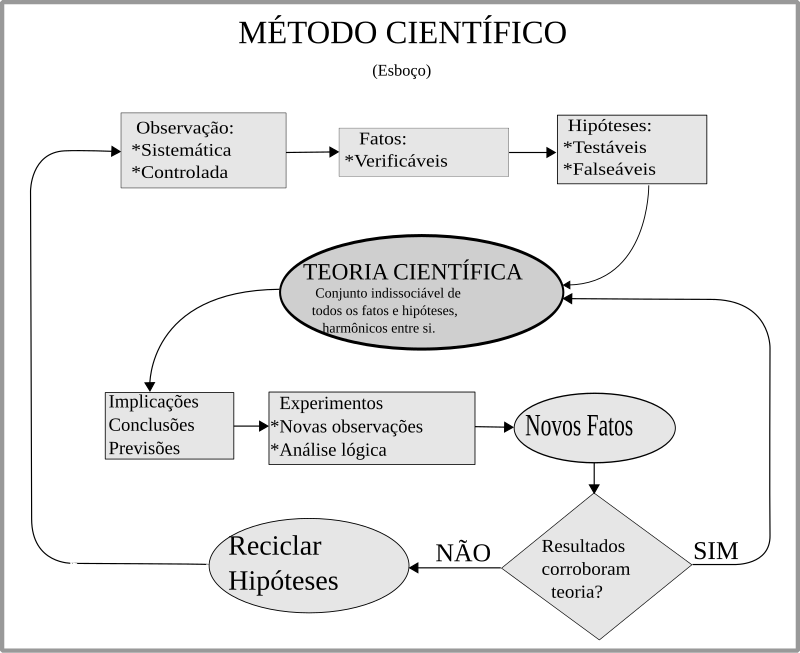
\includegraphics[width=0.6\textwidth]{figuras/metodo_cientifico.png}
	% Caption centralizada
% 	\captionsetup{justification=centering}
	% Caption e fonte 
	 \vspace{-0.2cm}
	\\\textbf{\footnotesize Fonte: Wikipédia }
	\label{fig:figura1}
\end{figure}
\vspace{-0.5cm}


   
\section{\esp CONCLUSÃO}

A classificação lógica da pesquisa em exploratória, descritiva e explicativa representa não apenas uma organização didática do conhecimento metodológico, mas também uma estratégia prática fundamental para a condução científica eficaz. A pesquisa exploratória permite ao pesquisador identificar caminhos e construir bases iniciais sólidas; a pesquisa descritiva oferece um retrato fiel da realidade observada, permitindo comparações e formulações iniciais de padrões; e a pesquisa explicativa propicia o aprofundamento na compreensão dos fenômenos, estabelecendo relações causais que contribuem para o avanço da ciência.

A escolha adequada do tipo de pesquisa a ser realizado deve considerar a maturidade do tema estudado, os objetivos científicos do estudo e as possibilidades metodológicas disponíveis. Mais do que uma escolha técnica, trata-se de uma decisão estratégica que impacta diretamente na qualidade dos dados obtidos e na robustez das conclusões. Assim, conhecer profundamente as características, potencialidades e limitações de cada tipo lógico de pesquisa é condição sine qua non para o desenvolvimento de estudos científicos relevantes, inovadores e socialmente úteis.

\nocite{artigo01}
\nocite{artigo02}
\nocite{artigo03}
\nocite{videoaula}





% \subsection{\esp Trabalhos futuros}
% 
% Sugestões de estudos posteriores são ser adicionados subseção deste capítulo de conclusão.


%%%%%%%%%%%%%%%%%%%%%%%%%%%%%%%%%%%
%% FIM DO TEXTO
%%%%%%%%%%%%%%%%%%%%%%%%%%%%%%%%%%%

% \selectlanguage{brazil}
%%%%%%%%%%%%%%%%%%%%%%%%%%%%%%%%%%%
%% Inicio bibliografia
%%%%%%%%%%%%%%%%%%%%%%%%%%%%%%%%%%%

 \newpage
\singlespace{
\renewcommand\refname{REFERÊNCIAS}
\bibliographystyle{abntex2-alf}
\bibliography{bibliografia}

}

\end{document}


